\documentclass[twoside]{book}

% Packages required by doxygen
\usepackage{calc}
\usepackage{doxygen}
\usepackage{graphicx}
\usepackage[utf8]{inputenc}
\usepackage{makeidx}
\usepackage{multicol}
\usepackage{multirow}
\usepackage{textcomp}
\usepackage[table]{xcolor}

% Font selection
\usepackage[T1]{fontenc}
\usepackage{mathptmx}
\usepackage[scaled=.90]{helvet}
\usepackage{courier}
\usepackage{amssymb}
\usepackage{sectsty}
\renewcommand{\familydefault}{\sfdefault}
\allsectionsfont{%
  \fontseries{bc}\selectfont%
  \color{darkgray}%
}
\renewcommand{\DoxyLabelFont}{%
  \fontseries{bc}\selectfont%
  \color{darkgray}%
}

% Page & text layout
\usepackage{geometry}
\geometry{%
  a4paper,%
  top=2.5cm,%
  bottom=2.5cm,%
  left=2.5cm,%
  right=2.5cm%
}
\tolerance=750
\hfuzz=15pt
\hbadness=750
\setlength{\emergencystretch}{15pt}
\setlength{\parindent}{0cm}
\setlength{\parskip}{0.2cm}
\makeatletter
\renewcommand{\paragraph}{%
  \@startsection{paragraph}{4}{0ex}{-1.0ex}{1.0ex}{%
    \normalfont\normalsize\bfseries\SS@parafont%
  }%
}
\renewcommand{\subparagraph}{%
  \@startsection{subparagraph}{5}{0ex}{-1.0ex}{1.0ex}{%
    \normalfont\normalsize\bfseries\SS@subparafont%
  }%
}
\makeatother

% Headers & footers
\usepackage{fancyhdr}
\pagestyle{fancyplain}
\fancyhead[LE]{\fancyplain{}{\bfseries\thepage}}
\fancyhead[CE]{\fancyplain{}{}}
\fancyhead[RE]{\fancyplain{}{\bfseries\leftmark}}
\fancyhead[LO]{\fancyplain{}{\bfseries\rightmark}}
\fancyhead[CO]{\fancyplain{}{}}
\fancyhead[RO]{\fancyplain{}{\bfseries\thepage}}
\fancyfoot[LE]{\fancyplain{}{}}
\fancyfoot[CE]{\fancyplain{}{}}
\fancyfoot[RE]{\fancyplain{}{\bfseries\scriptsize Generated on Mon Feb 17 2014 08\-:00\-:18 for Dopple\-Scanner by Doxygen }}
\fancyfoot[LO]{\fancyplain{}{\bfseries\scriptsize Generated on Mon Feb 17 2014 08\-:00\-:18 for Dopple\-Scanner by Doxygen }}
\fancyfoot[CO]{\fancyplain{}{}}
\fancyfoot[RO]{\fancyplain{}{}}
\renewcommand{\footrulewidth}{0.4pt}
\renewcommand{\chaptermark}[1]{%
  \markboth{#1}{}%
}
\renewcommand{\sectionmark}[1]{%
  \markright{\thesection\ #1}%
}

% Indices & bibliography
\usepackage{natbib}
\usepackage[titles]{tocloft}
\setcounter{tocdepth}{3}
\setcounter{secnumdepth}{5}
\makeindex

% Hyperlinks (required, but should be loaded last)
\usepackage{ifpdf}
\ifpdf
  \usepackage[pdftex,pagebackref=true]{hyperref}
\else
  \usepackage[ps2pdf,pagebackref=true]{hyperref}
\fi
\hypersetup{%
  colorlinks=true,%
  linkcolor=blue,%
  citecolor=blue,%
  unicode%
}

% Custom commands
\newcommand{\clearemptydoublepage}{%
  \newpage{\pagestyle{empty}\cleardoublepage}%
}


%===== C O N T E N T S =====

\begin{document}

% Titlepage & ToC
\hypersetup{pageanchor=false}
\pagenumbering{roman}
\begin{titlepage}
\vspace*{7cm}
\begin{center}%
{\Large Dopple\-Scanner }\\
\vspace*{1cm}
{\large Generated by Doxygen 1.8.6}\\
\vspace*{0.5cm}
{\small Mon Feb 17 2014 08:00:18}\\
\end{center}
\end{titlepage}
\clearemptydoublepage
\tableofcontents
\clearemptydoublepage
\pagenumbering{arabic}
\hypersetup{pageanchor=true}

%--- Begin generated contents ---
\chapter{Hierarchical Index}
\section{Class Hierarchy}
This inheritance list is sorted roughly, but not completely, alphabetically\-:\begin{DoxyCompactList}
\item Q\-Main\-Window\begin{DoxyCompactList}
\item \contentsline{section}{Main\-Window}{\pageref{class_main_window}}{}
\end{DoxyCompactList}
\item \contentsline{section}{qt\-\_\-meta\-\_\-stringdata\-\_\-\-Main\-Window\-\_\-t}{\pageref{structqt__meta__stringdata___main_window__t}}{}
\item \contentsline{section}{S\-H\-A1}{\pageref{class_s_h_a1}}{}
\item \contentsline{section}{Tree\-Scanner}{\pageref{class_tree_scanner}}{}
\item \contentsline{section}{Ui\-\_\-\-Main\-Window}{\pageref{class_ui___main_window}}{}
\begin{DoxyCompactList}
\item \contentsline{section}{Ui\-:\-:Main\-Window}{\pageref{class_ui_1_1_main_window}}{}
\item \contentsline{section}{Ui\-:\-:Main\-Window}{\pageref{class_ui_1_1_main_window}}{}
\end{DoxyCompactList}
\item \contentsline{section}{User\-Interface}{\pageref{class_user_interface}}{}
\end{DoxyCompactList}

\chapter{Class Index}
\section{Class List}
Here are the classes, structs, unions and interfaces with brief descriptions\-:\begin{DoxyCompactList}
\item\contentsline{section}{\hyperlink{class_ui_1_1_main_window}{Ui\-::\-Main\-Window} }{\pageref{class_ui_1_1_main_window}}{}
\item\contentsline{section}{\hyperlink{class_main_window}{Main\-Window} }{\pageref{class_main_window}}{}
\item\contentsline{section}{\hyperlink{structqt__meta__stringdata___main_window__t}{qt\-\_\-meta\-\_\-stringdata\-\_\-\-Main\-Window\-\_\-t} }{\pageref{structqt__meta__stringdata___main_window__t}}{}
\item\contentsline{section}{\hyperlink{class_s_h_a1}{S\-H\-A1} }{\pageref{class_s_h_a1}}{}
\item\contentsline{section}{\hyperlink{class_tree_scanner}{Tree\-Scanner} }{\pageref{class_tree_scanner}}{}
\item\contentsline{section}{\hyperlink{class_ui___main_window}{Ui\-\_\-\-Main\-Window} }{\pageref{class_ui___main_window}}{}
\item\contentsline{section}{\hyperlink{class_user_interface}{User\-Interface} }{\pageref{class_user_interface}}{}
\end{DoxyCompactList}

\chapter{Class Documentation}
\hypertarget{class_ui_1_1_main_window}{\section{Ui\-:\-:Main\-Window Class Reference}
\label{class_ui_1_1_main_window}\index{Ui\-::\-Main\-Window@{Ui\-::\-Main\-Window}}
}
Inheritance diagram for Ui\-:\-:Main\-Window\-:\begin{figure}[H]
\begin{center}
\leavevmode
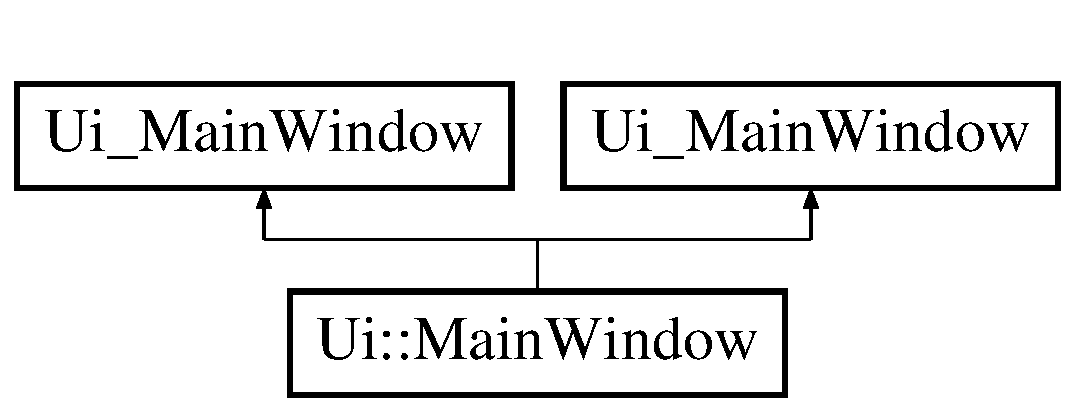
\includegraphics[height=2.000000cm]{class_ui_1_1_main_window}
\end{center}
\end{figure}
\subsection*{Additional Inherited Members}


The documentation for this class was generated from the following file\-:\begin{DoxyCompactItemize}
\item 
E\-:/duplicates/\-Source/\-S\-D2013\-D\-Scanner/build-\/\-Dopple\-Scanner3-\/\-Desktop\-\_\-\-Qt\-\_\-5\-\_\-2\-\_\-1\-\_\-\-Min\-G\-W\-\_\-32bit-\/\-Debug/ui\-\_\-mainwindow.\-h\end{DoxyCompactItemize}

\hypertarget{class_main_window}{\section{Main\-Window Class Reference}
\label{class_main_window}\index{Main\-Window@{Main\-Window}}
}
Inheritance diagram for Main\-Window\-:\begin{figure}[H]
\begin{center}
\leavevmode
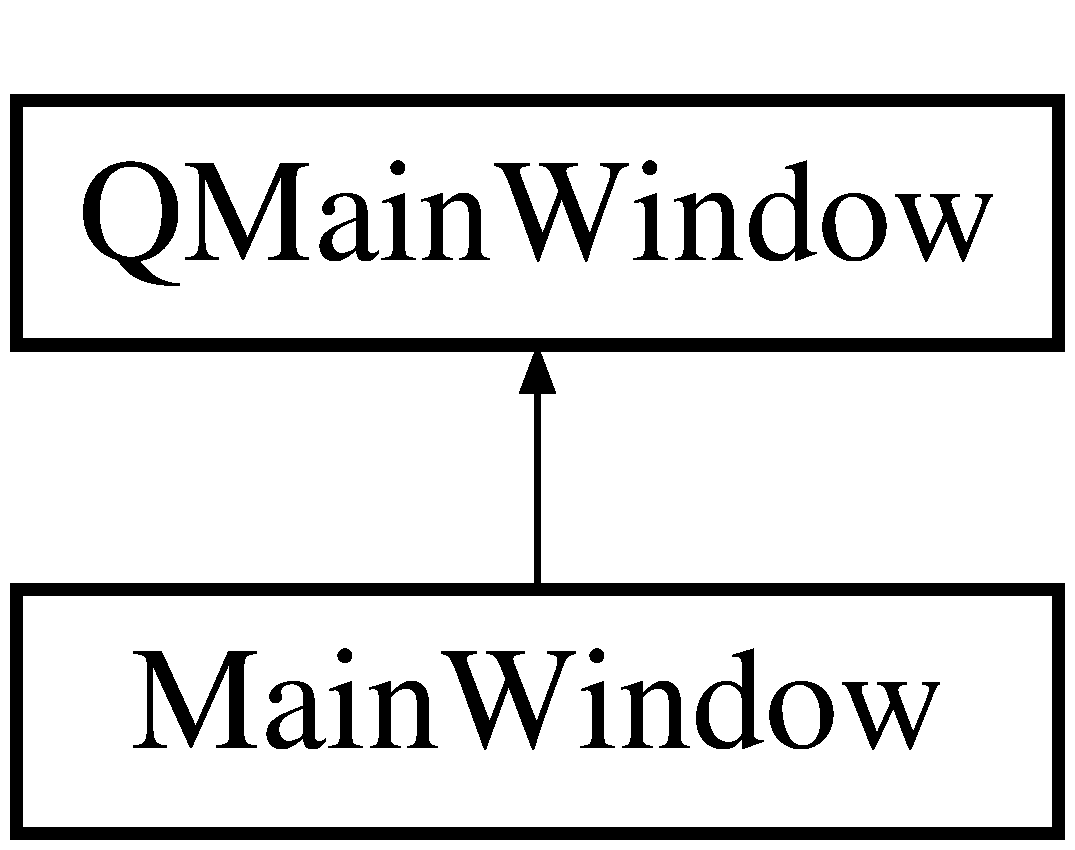
\includegraphics[height=2.000000cm]{class_main_window}
\end{center}
\end{figure}
\subsection*{Public Member Functions}
\begin{DoxyCompactItemize}
\item 
\hypertarget{class_main_window_a8b244be8b7b7db1b08de2a2acb9409db}{{\bfseries Main\-Window} (Q\-Widget $\ast$parent=0)}\label{class_main_window_a8b244be8b7b7db1b08de2a2acb9409db}

\end{DoxyCompactItemize}


The documentation for this class was generated from the following files\-:\begin{DoxyCompactItemize}
\item 
E\-:/duplicates/\-Source/\-S\-D2013\-D\-Scanner/\-Dopple\-Scanner3/mainwindow.\-h\item 
E\-:/duplicates/\-Source/\-S\-D2013\-D\-Scanner/\-Dopple\-Scanner3/mainwindow.\-cpp\end{DoxyCompactItemize}

\hypertarget{structqt__meta__stringdata___main_window__t}{\section{qt\-\_\-meta\-\_\-stringdata\-\_\-\-Main\-Window\-\_\-t Struct Reference}
\label{structqt__meta__stringdata___main_window__t}\index{qt\-\_\-meta\-\_\-stringdata\-\_\-\-Main\-Window\-\_\-t@{qt\-\_\-meta\-\_\-stringdata\-\_\-\-Main\-Window\-\_\-t}}
}
\subsection*{Public Attributes}
\begin{DoxyCompactItemize}
\item 
\hypertarget{structqt__meta__stringdata___main_window__t_af598c0b01c666753185a38017d12d5cc}{Q\-Byte\-Array\-Data {\bfseries data} \mbox{[}6\mbox{]}}\label{structqt__meta__stringdata___main_window__t_af598c0b01c666753185a38017d12d5cc}

\item 
\hypertarget{structqt__meta__stringdata___main_window__t_a827a4cb99dff5edec6d535a58462376c}{char {\bfseries stringdata} \mbox{[}92\mbox{]}}\label{structqt__meta__stringdata___main_window__t_a827a4cb99dff5edec6d535a58462376c}

\end{DoxyCompactItemize}


The documentation for this struct was generated from the following file\-:\begin{DoxyCompactItemize}
\item 
E\-:/duplicates/\-Source/\-S\-D2013\-D\-Scanner/build-\/\-Dopple\-Scanner3-\/\-Desktop\-\_\-\-Qt\-\_\-5\-\_\-2\-\_\-1\-\_\-\-Min\-G\-W\-\_\-32bit-\/\-Debug/debug/moc\-\_\-mainwindow.\-cpp\end{DoxyCompactItemize}

\hypertarget{class_s_h_a1}{\section{S\-H\-A1 Class Reference}
\label{class_s_h_a1}\index{S\-H\-A1@{S\-H\-A1}}
}
\subsection*{Public Member Functions}
\begin{DoxyCompactItemize}
\item 
\hypertarget{class_s_h_a1_aec3a46058baf8b4169389c89e3a0a2f4}{void {\bfseries update} (const std\-::string \&s)}\label{class_s_h_a1_aec3a46058baf8b4169389c89e3a0a2f4}

\item 
\hypertarget{class_s_h_a1_a71d172f1d0b34c5a381ccdfce5aa6ab5}{void {\bfseries update} (std\-::istream \&is)}\label{class_s_h_a1_a71d172f1d0b34c5a381ccdfce5aa6ab5}

\item 
\hypertarget{class_s_h_a1_a89ba0f16575431b0942cbbcfb29107db}{std\-::string {\bfseries final} ()}\label{class_s_h_a1_a89ba0f16575431b0942cbbcfb29107db}

\item 
\hypertarget{class_s_h_a1_aec3a46058baf8b4169389c89e3a0a2f4}{void {\bfseries update} (const std\-::string \&s)}\label{class_s_h_a1_aec3a46058baf8b4169389c89e3a0a2f4}

\item 
\hypertarget{class_s_h_a1_a71d172f1d0b34c5a381ccdfce5aa6ab5}{void {\bfseries update} (std\-::istream \&is)}\label{class_s_h_a1_a71d172f1d0b34c5a381ccdfce5aa6ab5}

\item 
\hypertarget{class_s_h_a1_a89ba0f16575431b0942cbbcfb29107db}{std\-::string {\bfseries final} ()}\label{class_s_h_a1_a89ba0f16575431b0942cbbcfb29107db}

\end{DoxyCompactItemize}
\subsection*{Static Public Member Functions}
\begin{DoxyCompactItemize}
\item 
\hypertarget{class_s_h_a1_a1bec6fb50bcfb5e3f6fb5c8f258a1f41}{static std\-::string {\bfseries from\-\_\-file} (const std\-::string \&filename)}\label{class_s_h_a1_a1bec6fb50bcfb5e3f6fb5c8f258a1f41}

\item 
\hypertarget{class_s_h_a1_a72ef6f0f4c3e6a2a9d751031d3014c53}{static std\-::string {\bfseries from\-\_\-file} (const std\-::string \&filename)}\label{class_s_h_a1_a72ef6f0f4c3e6a2a9d751031d3014c53}

\end{DoxyCompactItemize}


The documentation for this class was generated from the following files\-:\begin{DoxyCompactItemize}
\item 
E\-:/duplicates/\-Source/\-S\-D2013\-D\-Scanner/\-Dopple\-Scanner3/sha1.\-h\item 
E\-:/duplicates/\-Source/\-S\-D2013\-D\-Scanner/\-Dopple\-Scanner3/sha1.\-cpp\end{DoxyCompactItemize}

\hypertarget{class_tree_scanner}{\section{Tree\-Scanner Class Reference}
\label{class_tree_scanner}\index{Tree\-Scanner@{Tree\-Scanner}}
}
\subsection*{Public Member Functions}
\begin{DoxyCompactItemize}
\item 
bool \hyperlink{class_tree_scanner_ae00aada3fc132df9c016b929cf28c9bc}{Is\-File} (const string \&path)
\item 
\hypertarget{class_tree_scanner_aa7b2ea3b785abfeb7947fdd74ce64953}{bool \hyperlink{class_tree_scanner_aa7b2ea3b785abfeb7947fdd74ce64953}{Is\-Directory} (const string \&path)}\label{class_tree_scanner_aa7b2ea3b785abfeb7947fdd74ce64953}

\begin{DoxyCompactList}\small\item\em Checks whether the given absolute or relative path is a valid directory. \end{DoxyCompactList}\item 
size\-\_\-t \hyperlink{class_tree_scanner_af9f6d985cb42d2cd7505b1213edd04b8}{File\-Size\-In\-Bytes} (const string \&filename)
\item 
vector$<$ string $>$ \hyperlink{class_tree_scanner_a1ad8ab7b22690ae99f25e9b26ab31f6d}{Get\-Files\-And\-Directories\-Flat} (const string \&directory)
\begin{DoxyCompactList}\small\item\em given directory specified by its absolute or relative path. \end{DoxyCompactList}\item 
void \hyperlink{class_tree_scanner_a042ddf3be0d3960dbca0362fb52cd1cd}{Get\-Files\-And\-Directories\-Recursive} (const string \&base\-\_\-path, vector$<$ string $>$ \&files\-\_\-and\-\_\-directories)
\item 
void \hyperlink{class_tree_scanner_add67141b6bca7a3abc72ea305ac915bd}{Group\-Into\-Classes} (const string \&base\-\_\-directory, map$<$ string, vector$<$ string $>$ $>$ \&classes)
\end{DoxyCompactItemize}


\subsection{Member Function Documentation}
\hypertarget{class_tree_scanner_af9f6d985cb42d2cd7505b1213edd04b8}{\index{Tree\-Scanner@{Tree\-Scanner}!File\-Size\-In\-Bytes@{File\-Size\-In\-Bytes}}
\index{File\-Size\-In\-Bytes@{File\-Size\-In\-Bytes}!TreeScanner@{Tree\-Scanner}}
\subsubsection[{File\-Size\-In\-Bytes}]{\setlength{\rightskip}{0pt plus 5cm}size\-\_\-t Tree\-Scanner\-::\-File\-Size\-In\-Bytes (
\begin{DoxyParamCaption}
\item[{const string \&}]{filename}
\end{DoxyParamCaption}
)}}\label{class_tree_scanner_af9f6d985cb42d2cd7505b1213edd04b8}
A method that estimates the size of a file 
\begin{DoxyParams}{Parameters}
{\em filename} & A constant reference to a string of a filename \\
\hline
\end{DoxyParams}
\begin{DoxyReturn}{Returns}
The number of bytes the given file contains. 
\end{DoxyReturn}
\hypertarget{class_tree_scanner_a1ad8ab7b22690ae99f25e9b26ab31f6d}{\index{Tree\-Scanner@{Tree\-Scanner}!Get\-Files\-And\-Directories\-Flat@{Get\-Files\-And\-Directories\-Flat}}
\index{Get\-Files\-And\-Directories\-Flat@{Get\-Files\-And\-Directories\-Flat}!TreeScanner@{Tree\-Scanner}}
\subsubsection[{Get\-Files\-And\-Directories\-Flat}]{\setlength{\rightskip}{0pt plus 5cm}vector$<$ string $>$ Tree\-Scanner\-::\-Get\-Files\-And\-Directories\-Flat (
\begin{DoxyParamCaption}
\item[{const string \&}]{directory}
\end{DoxyParamCaption}
)}}\label{class_tree_scanner_a1ad8ab7b22690ae99f25e9b26ab31f6d}


given directory specified by its absolute or relative path. 

Returns the names of all files and directories directly contained in a


\begin{DoxyParams}{Parameters}
{\em directory} & a string to the main directory. \\
\hline
\end{DoxyParams}
\begin{DoxyReturn}{Returns}
Returns the names of all files and directories directly or indirectly (recursively) contained in a given directory specified by it's absolute or relative path. The names are stored in the output parameter\-: files\-\_\-and\-\_\-directories and are included using an in-\/order traversal of the filesystem.. 
\end{DoxyReturn}
\hypertarget{class_tree_scanner_a042ddf3be0d3960dbca0362fb52cd1cd}{\index{Tree\-Scanner@{Tree\-Scanner}!Get\-Files\-And\-Directories\-Recursive@{Get\-Files\-And\-Directories\-Recursive}}
\index{Get\-Files\-And\-Directories\-Recursive@{Get\-Files\-And\-Directories\-Recursive}!TreeScanner@{Tree\-Scanner}}
\subsubsection[{Get\-Files\-And\-Directories\-Recursive}]{\setlength{\rightskip}{0pt plus 5cm}void Tree\-Scanner\-::\-Get\-Files\-And\-Directories\-Recursive (
\begin{DoxyParamCaption}
\item[{const string \&}]{base\-\_\-path, }
\item[{vector$<$ string $>$ \&}]{files\-\_\-and\-\_\-directories}
\end{DoxyParamCaption}
)}}\label{class_tree_scanner_a042ddf3be0d3960dbca0362fb52cd1cd}
Recursive version of Get\-Files\-And\-Directories\-Flat(...) \begin{DoxySeeAlso}{See Also}
\hyperlink{class_tree_scanner_a1ad8ab7b22690ae99f25e9b26ab31f6d}{Get\-Files\-And\-Directories\-Flat()} 
\end{DoxySeeAlso}

\begin{DoxyParams}{Parameters}
{\em base\-\_\-path} & A constant reference to a string a base path \\
\hline
{\em files\-\_\-and\-\_\-directories} & A reference to a vector of strings of filenames and the paths to them \\
\hline
\end{DoxyParams}
\hypertarget{class_tree_scanner_add67141b6bca7a3abc72ea305ac915bd}{\index{Tree\-Scanner@{Tree\-Scanner}!Group\-Into\-Classes@{Group\-Into\-Classes}}
\index{Group\-Into\-Classes@{Group\-Into\-Classes}!TreeScanner@{Tree\-Scanner}}
\subsubsection[{Group\-Into\-Classes}]{\setlength{\rightskip}{0pt plus 5cm}void Tree\-Scanner\-::\-Group\-Into\-Classes (
\begin{DoxyParamCaption}
\item[{const string \&}]{base\-\_\-directory, }
\item[{map$<$ string, vector$<$ string $>$ $>$ \&}]{classes}
\end{DoxyParamCaption}
)}}\label{class_tree_scanner_add67141b6bca7a3abc72ea305ac915bd}
Recursively traverses the files in a base directory and creates a map from hashes of file contents to a vector of filenames. This results in a grouping in which the names of all files with the same content are put into the same vector. \hypertarget{class_tree_scanner_ae00aada3fc132df9c016b929cf28c9bc}{\index{Tree\-Scanner@{Tree\-Scanner}!Is\-File@{Is\-File}}
\index{Is\-File@{Is\-File}!TreeScanner@{Tree\-Scanner}}
\subsubsection[{Is\-File}]{\setlength{\rightskip}{0pt plus 5cm}bool Tree\-Scanner\-::\-Is\-File (
\begin{DoxyParamCaption}
\item[{const string \&}]{path}
\end{DoxyParamCaption}
)}}\label{class_tree_scanner_ae00aada3fc132df9c016b929cf28c9bc}
Checks whether the given absolute or relative path is a valid file. 
\begin{DoxyParams}{Parameters}
{\em path} & A constant reference to a string of a path \\
\hline
\end{DoxyParams}
\begin{DoxyReturn}{Returns}
A whether the string is a path to a file 
\end{DoxyReturn}


The documentation for this class was generated from the following files\-:\begin{DoxyCompactItemize}
\item 
E\-:/duplicates/\-Source/\-S\-D2013\-D\-Scanner/Tree\-Scanner.\-h\item 
E\-:/duplicates/\-Source/\-S\-D2013\-D\-Scanner/Tree\-Scanner.\-cpp\end{DoxyCompactItemize}

\hypertarget{class_ui___main_window}{\section{Ui\-\_\-\-Main\-Window Class Reference}
\label{class_ui___main_window}\index{Ui\-\_\-\-Main\-Window@{Ui\-\_\-\-Main\-Window}}
}
Inheritance diagram for Ui\-\_\-\-Main\-Window\-:\begin{figure}[H]
\begin{center}
\leavevmode
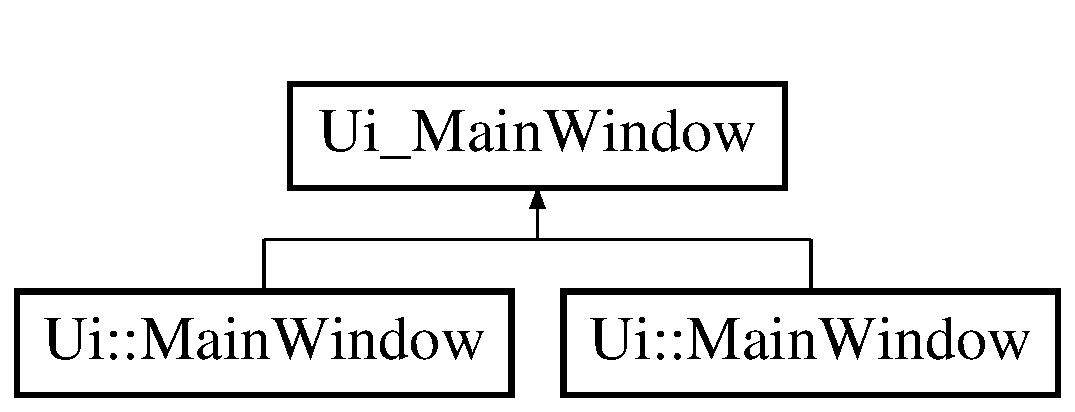
\includegraphics[height=2.000000cm]{class_ui___main_window}
\end{center}
\end{figure}
\subsection*{Public Member Functions}
\begin{DoxyCompactItemize}
\item 
\hypertarget{class_ui___main_window_acf4a0872c4c77d8f43a2ec66ed849b58}{void {\bfseries setup\-Ui} (Q\-Main\-Window $\ast$\hyperlink{class_main_window}{Main\-Window})}\label{class_ui___main_window_acf4a0872c4c77d8f43a2ec66ed849b58}

\item 
\hypertarget{class_ui___main_window_a097dd160c3534a204904cb374412c618}{void {\bfseries retranslate\-Ui} (Q\-Main\-Window $\ast$\hyperlink{class_main_window}{Main\-Window})}\label{class_ui___main_window_a097dd160c3534a204904cb374412c618}

\item 
\hypertarget{class_ui___main_window_acf4a0872c4c77d8f43a2ec66ed849b58}{void {\bfseries setup\-Ui} (Q\-Main\-Window $\ast$\hyperlink{class_main_window}{Main\-Window})}\label{class_ui___main_window_acf4a0872c4c77d8f43a2ec66ed849b58}

\item 
\hypertarget{class_ui___main_window_a097dd160c3534a204904cb374412c618}{void {\bfseries retranslate\-Ui} (Q\-Main\-Window $\ast$\hyperlink{class_main_window}{Main\-Window})}\label{class_ui___main_window_a097dd160c3534a204904cb374412c618}

\end{DoxyCompactItemize}
\subsection*{Public Attributes}
\begin{DoxyCompactItemize}
\item 
\hypertarget{class_ui___main_window_a6600dd3bdd3d55e535659e4a4096ea48}{Q\-Widget $\ast$ {\bfseries central\-Widget}}\label{class_ui___main_window_a6600dd3bdd3d55e535659e4a4096ea48}

\item 
\hypertarget{class_ui___main_window_a649287f742c9a33b8444116dccb1b72b}{Q\-V\-Box\-Layout $\ast$ {\bfseries vertical\-Layout}}\label{class_ui___main_window_a649287f742c9a33b8444116dccb1b72b}

\item 
\hypertarget{class_ui___main_window_a9ee21d2c2bc000e7a8ba931bacfc5a69}{Q\-H\-Box\-Layout $\ast$ {\bfseries horizontal\-Layout\-\_\-2}}\label{class_ui___main_window_a9ee21d2c2bc000e7a8ba931bacfc5a69}

\item 
\hypertarget{class_ui___main_window_a2f5576686ce98bcc41bd1b1eca07e56a}{Q\-Label $\ast$ {\bfseries label\-\_\-2}}\label{class_ui___main_window_a2f5576686ce98bcc41bd1b1eca07e56a}

\item 
\hypertarget{class_ui___main_window_a8d1e96b1497ab37325c7cae014c2f31a}{Q\-Check\-Box $\ast$ {\bfseries master\-Check}}\label{class_ui___main_window_a8d1e96b1497ab37325c7cae014c2f31a}

\item 
\hypertarget{class_ui___main_window_a313ee66c70f96846198ea4a165cb9001}{Q\-Table\-Widget $\ast$ {\bfseries table\-Widget}}\label{class_ui___main_window_a313ee66c70f96846198ea4a165cb9001}

\item 
\hypertarget{class_ui___main_window_abc1222aa546de4fdd85fac3650d12787}{Q\-Push\-Button $\ast$ {\bfseries delete\-Button}}\label{class_ui___main_window_abc1222aa546de4fdd85fac3650d12787}

\item 
\hypertarget{class_ui___main_window_ae7104d878681f568e492c5bd0f653157}{Q\-H\-Box\-Layout $\ast$ {\bfseries horizontal\-Layout}}\label{class_ui___main_window_ae7104d878681f568e492c5bd0f653157}

\item 
\hypertarget{class_ui___main_window_a78edcdd12ea78c06d7e80f322c8882f9}{Q\-Label $\ast$ {\bfseries label}}\label{class_ui___main_window_a78edcdd12ea78c06d7e80f322c8882f9}

\item 
\hypertarget{class_ui___main_window_ac01f7b29def5868964d57473a693defe}{Q\-Line\-Edit $\ast$ {\bfseries path\-Input}}\label{class_ui___main_window_ac01f7b29def5868964d57473a693defe}

\item 
\hypertarget{class_ui___main_window_a41ca895e951c2e2f3c09deea57bd34c3}{Q\-Push\-Button $\ast$ {\bfseries scan\-Button}}\label{class_ui___main_window_a41ca895e951c2e2f3c09deea57bd34c3}

\item 
\hypertarget{class_ui___main_window_a502a50d7dc22415f511336bdfb4318b9}{Q\-Menu\-Bar $\ast$ {\bfseries menu\-Bar}}\label{class_ui___main_window_a502a50d7dc22415f511336bdfb4318b9}

\item 
\hypertarget{class_ui___main_window_abca26371605d7c5235fab5188d4bdcf7}{Q\-Tool\-Bar $\ast$ {\bfseries main\-Tool\-Bar}}\label{class_ui___main_window_abca26371605d7c5235fab5188d4bdcf7}

\item 
\hypertarget{class_ui___main_window_afa919f3af6f2f526a70f1fa331f63724}{Q\-Status\-Bar $\ast$ {\bfseries status\-Bar}}\label{class_ui___main_window_afa919f3af6f2f526a70f1fa331f63724}

\end{DoxyCompactItemize}


The documentation for this class was generated from the following file\-:\begin{DoxyCompactItemize}
\item 
E\-:/duplicates/\-Source/\-S\-D2013\-D\-Scanner/build-\/\-Dopple\-Scanner3-\/\-Desktop\-\_\-\-Qt\-\_\-5\-\_\-2\-\_\-1\-\_\-\-Min\-G\-W\-\_\-32bit-\/\-Debug/ui\-\_\-mainwindow.\-h\end{DoxyCompactItemize}

\hypertarget{class_user_interface}{\section{User\-Interface Class Reference}
\label{class_user_interface}\index{User\-Interface@{User\-Interface}}
}


{\ttfamily \#include $<$User\-Interface.\-h$>$}

\subsection*{Public Member Functions}
\begin{DoxyCompactItemize}
\item 
void \hyperlink{class_user_interface_a8ed960186e9c41fd8367b3d71da546f8}{output} (map$<$ string, vector$<$ string $>$ $>$ \&classes)
\item 
void \hyperlink{class_user_interface_ad27a5035bcd5d32eaf2ca870e8ab10a7}{output\-\_\-h} (map$<$ string, vector$<$ string $>$ $>$ \&classes)
\item 
void \hyperlink{class_user_interface_a62000ec96ec57056f5b6e6a6fcbfc719}{delete\-File} (string fname)
\item 
void \hyperlink{class_user_interface_afb94642309072d3927dac399afd744c2}{delete\-Duplicates} (map$<$ string, vector$<$ string $>$ $>$ \&classes, char token)
\item 
void \hyperlink{class_user_interface_aec96db5035550670c88f077d36b7ef24}{qt\-Output} (map$<$ string, vector$<$ string $>$ $>$ \&classes, Q\-String $\ast$\hyperlink{class_user_interface_a8ed960186e9c41fd8367b3d71da546f8}{output}, Q\-Table\-Widget $\ast$table)
\item 
void \hyperlink{class_user_interface_a8ed960186e9c41fd8367b3d71da546f8}{output} (map$<$ string, vector$<$ string $>$ $>$ \&classes)
\item 
\hypertarget{class_user_interface_ad27a5035bcd5d32eaf2ca870e8ab10a7}{void {\bfseries output\-\_\-h} (map$<$ string, vector$<$ string $>$ $>$ \&classes)}\label{class_user_interface_ad27a5035bcd5d32eaf2ca870e8ab10a7}

\item 
void \hyperlink{class_user_interface_afb94642309072d3927dac399afd744c2}{delete\-Duplicates} (map$<$ string, vector$<$ string $>$ $>$ \&classes, char token)
\end{DoxyCompactItemize}


\subsection{Detailed Description}
Constructs the user interface and contains. the different types ot output and input forms. 

\subsection{Member Function Documentation}
\hypertarget{class_user_interface_afb94642309072d3927dac399afd744c2}{\index{User\-Interface@{User\-Interface}!delete\-Duplicates@{delete\-Duplicates}}
\index{delete\-Duplicates@{delete\-Duplicates}!UserInterface@{User\-Interface}}
\subsubsection[{delete\-Duplicates}]{\setlength{\rightskip}{0pt plus 5cm}void User\-Interface\-::delete\-Duplicates (
\begin{DoxyParamCaption}
\item[{map$<$ string, vector$<$ string $>$ $>$ \&}]{classes, }
\item[{char}]{token}
\end{DoxyParamCaption}
)}}\label{class_user_interface_afb94642309072d3927dac399afd744c2}
Deletes a group of duplicates except one chosen by the user. 
\begin{DoxyParams}{Parameters}
{\em class\-\_\-cnt} & Keeps count of how many duplicates groups there are. \\
\hline
{\em token} & H\-T\-M\-L/\-C\-M\-D mode token. \\
\hline
\end{DoxyParams}
\hypertarget{class_user_interface_afb94642309072d3927dac399afd744c2}{\index{User\-Interface@{User\-Interface}!delete\-Duplicates@{delete\-Duplicates}}
\index{delete\-Duplicates@{delete\-Duplicates}!UserInterface@{User\-Interface}}
\subsubsection[{delete\-Duplicates}]{\setlength{\rightskip}{0pt plus 5cm}void User\-Interface\-::delete\-Duplicates (
\begin{DoxyParamCaption}
\item[{map$<$ string, vector$<$ string $>$ $>$ \&}]{classes, }
\item[{char}]{token}
\end{DoxyParamCaption}
)}}\label{class_user_interface_afb94642309072d3927dac399afd744c2}
Deletes a group of duplicates except one chosen by the user. 
\begin{DoxyParams}{Parameters}
{\em class\-\_\-cnt} & Keeps count of how many duplicates groups there are. \\
\hline
{\em token} & H\-T\-M\-L/\-C\-M\-D mode token. \\
\hline
\end{DoxyParams}
\hypertarget{class_user_interface_a62000ec96ec57056f5b6e6a6fcbfc719}{\index{User\-Interface@{User\-Interface}!delete\-File@{delete\-File}}
\index{delete\-File@{delete\-File}!UserInterface@{User\-Interface}}
\subsubsection[{delete\-File}]{\setlength{\rightskip}{0pt plus 5cm}void User\-Interface\-::delete\-File (
\begin{DoxyParamCaption}
\item[{string}]{fname}
\end{DoxyParamCaption}
)}}\label{class_user_interface_a62000ec96ec57056f5b6e6a6fcbfc719}
Deletes a single file. 
\begin{DoxyParams}{Parameters}
{\em fname} & A string of a directory to a file. \\
\hline
\end{DoxyParams}
\hypertarget{class_user_interface_a8ed960186e9c41fd8367b3d71da546f8}{\index{User\-Interface@{User\-Interface}!output@{output}}
\index{output@{output}!UserInterface@{User\-Interface}}
\subsubsection[{output}]{\setlength{\rightskip}{0pt plus 5cm}void User\-Interface\-::output (
\begin{DoxyParamCaption}
\item[{map$<$ string, vector$<$ string $>$ $>$ \&}]{classes}
\end{DoxyParamCaption}
)}}\label{class_user_interface_a8ed960186e9c41fd8367b3d71da546f8}
Outputs the groups of duplicates in the command prompt. Shows the size consumed by duplicate files. 
\begin{DoxyParams}{Parameters}
{\em classes} & A map of strings and vectors of strings grouping files(directories) by their hash value. \\
\hline
\end{DoxyParams}
\hypertarget{class_user_interface_a8ed960186e9c41fd8367b3d71da546f8}{\index{User\-Interface@{User\-Interface}!output@{output}}
\index{output@{output}!UserInterface@{User\-Interface}}
\subsubsection[{output}]{\setlength{\rightskip}{0pt plus 5cm}void User\-Interface\-::output (
\begin{DoxyParamCaption}
\item[{map$<$ string, vector$<$ string $>$ $>$ \&}]{classes}
\end{DoxyParamCaption}
)}}\label{class_user_interface_a8ed960186e9c41fd8367b3d71da546f8}
Outputs the groups of duplicates in the command prompt. Shows the size consumed by duplicate files. 
\begin{DoxyParams}{Parameters}
{\em classes} & A map of strings and vectors of strings grouping files(directories) by their hash value. \\
\hline
\end{DoxyParams}
\hypertarget{class_user_interface_ad27a5035bcd5d32eaf2ca870e8ab10a7}{\index{User\-Interface@{User\-Interface}!output\-\_\-h@{output\-\_\-h}}
\index{output\-\_\-h@{output\-\_\-h}!UserInterface@{User\-Interface}}
\subsubsection[{output\-\_\-h}]{\setlength{\rightskip}{0pt plus 5cm}void User\-Interface\-::output\-\_\-h (
\begin{DoxyParamCaption}
\item[{map$<$ string, vector$<$ string $>$ $>$ \&}]{classes}
\end{DoxyParamCaption}
)}}\label{class_user_interface_ad27a5035bcd5d32eaf2ca870e8ab10a7}
H\-T\-M\-L version of \hyperlink{class_user_interface_a8ed960186e9c41fd8367b3d71da546f8}{output()}. \begin{DoxySeeAlso}{See Also}
\hyperlink{class_user_interface_a8ed960186e9c41fd8367b3d71da546f8}{output()} 
\end{DoxySeeAlso}
\hypertarget{class_user_interface_aec96db5035550670c88f077d36b7ef24}{\index{User\-Interface@{User\-Interface}!qt\-Output@{qt\-Output}}
\index{qt\-Output@{qt\-Output}!UserInterface@{User\-Interface}}
\subsubsection[{qt\-Output}]{\setlength{\rightskip}{0pt plus 5cm}void User\-Interface\-::qt\-Output (
\begin{DoxyParamCaption}
\item[{map$<$ string, vector$<$ string $>$ $>$ \&}]{classes, }
\item[{Q\-String $\ast$}]{output, }
\item[{Q\-Table\-Widget $\ast$}]{table}
\end{DoxyParamCaption}
)}}\label{class_user_interface_aec96db5035550670c88f077d36b7ef24}
Qt G\-U\-I version of \hyperlink{class_user_interface_a8ed960186e9c41fd8367b3d71da546f8}{output()}. \begin{DoxySeeAlso}{See Also}
\hyperlink{class_user_interface_a8ed960186e9c41fd8367b3d71da546f8}{output()} 
\end{DoxySeeAlso}

\begin{DoxyParams}{Parameters}
{\em table} & A Q\-Table\-Widget outputing the results from the scan into a table with a checkbox for deletion select. \\
\hline
\end{DoxyParams}


The documentation for this class was generated from the following files\-:\begin{DoxyCompactItemize}
\item 
E\-:/duplicates/\-Source/\-S\-D2013\-D\-Scanner/\-Dopple\-Scanner3/User\-Interface.\-h\item 
E\-:/duplicates/\-Source/\-S\-D2013\-D\-Scanner/\-Dopple\-Scanner3/User\-Interface.\-cpp\end{DoxyCompactItemize}

%--- End generated contents ---

% Index
\newpage
\phantomsection
\addcontentsline{toc}{chapter}{Index}
\printindex

\end{document}
